%% LaTeX2e class for seminar theses
%% seminar.tex
%% 
%% Karlsruhe Institute of Technology
%% Institute for Program Structures and Data Organization
%% Chair for Software Design and Quality (SDQ)
%%
%% Dr.-Ing. Erik Burger
%% burger@kit.edu
%%
%% Version 1.0.4, 2021-06-21

%% Available page modes: oneside, twoside
%% Available languages: english, ngerman
%% Available modes: draft, final (see README)
\documentclass[twoside, ngerman]{sdqseminar}

%% ---------------------------------
%% | Information about the thesis  |
%% ---------------------------------

%% Name of the author
\author{Alina Valta}

%% Title (and possibly subtitle) of the thesis
\title{Refaktorisierung einer Architekturanalyse für Vertraulichkeit}

%% Type of the thesis 
% \thesistype{Seminar Thesis}

%% Change the institute here, ``KASTEL'' is default
% \myinstitute{Institute for \dots}

%% The advisors are PhD Students or Postdocs
\advisor{M.Sc. Frederik Reiche}

\settitle

%% --------------------------------
%% | Settings for word separation |
%% --------------------------------

%% Describe separation hints here.
%% For more details, see 
%% http://en.wikibooks.org/wiki/LaTeX/Text_Formatting#Hyphenation
\hyphenation{
% me-ta-mo-del
}

%% --------------------------------
%% | Bibliography                 |
%% --------------------------------

%% Use biber instead of BibTeX, see README
\usepackage[citestyle=numeric,style=numeric,backend=biber]{biblatex}

\usepackage{listings}
\usepackage{svg}
\addbibresource{seminar.bib}

%% ====================================
%% ====================================
%% ||                                ||
%% || Beginning of the main document ||
%% ||                                ||
%% ====================================
%% ====================================
\begin{document}

%% Set PDF metadata
\setpdf

%% Set the title
\maketitle

%% ----------------
%% |   Abstract   |
%% ----------------
 
%% The text is included from the following files:
%% - sections/abstract

\begin{abstract}
%\input{sections/abstract.tex}
\end{abstract}

%% -----------------
%% |   Main part   |
%% -----------------


%\input{sections/introduction.tex}
%%% LaTeX2e class for seminar theses
%% sections/content.tex
%% 
%% Karlsruhe Institute of Technology
%% Institute for Program Structures and Data Organization
%% Chair for Software Design and Quality (SDQ)
%%
%% Dr.-Ing. Erik Burger
%% burger@kit.edu

\section{First Content Section}
\label{ch:FirstContentSection}

%% -------------------
%% | Example content |
%% -------------------
The content chapters of your thesis should of course be renamed. How many
chapters you need to write depends on your thesis and cannot be said in general.

Check out the examples theses in the SDQWiki:

\url{https://sdqweb.ipd.kit.edu/wiki/Form_der_Ausarbeitung_bei_Seminaren}

Of course, you can split this .tex file into several files if you prefer. 


\subsection{First Subsection}
\label{sec:FirstContentSection:FirstSubSection}

\dots

\subsection{A Subsection}
\label{sec:FirstContentSection:FirstSubSubSection}

\dots


\section{Second Content Section}
\label{ch:SecondContentSection}

\dots

\subsection{First Subsection}
\label{sec:SecondContentSection:FirstSubsection}

\dots

\subsection{Second Subsection}
\label{sec:SecondContentSection:SecondSubsection}

\dots

Add additional content sections if required by adding new .tex files in the
\code{sections/} directory and adding an appropriate 
\code{\textbackslash input} statement in \code{thesis.tex}. 
%% ---------------------
%% | / Example content |
%% ---------------------
%\input{sections/conclusion.tex}


\section{Aufgabenstellung}
Die Aufgabe dieses Praktikums ist eine Refaktorisierung der Projekte Confidentiality4CBSE\footnote{https://github.com/KASTEL-SCBS/Confidentiality4CBSE.git} und PCM2Prolog\footnote{https://github.com/KASTEL-SCBS/PCM2Prolog.git}. Die Aufgabe besteht dabei aus zwei Teilen: Die Entfernung des Profil-Mechanismus aus dem Confidentiality4CBSE Projekt und dem verfeinern des Modells, sodass der Informationsfluss genauer modelliert werden kann. Außerdem soll es sich bei dem Praktikum um eine Refaktorisierung handeln, weshalb der PCM2Prolog Generator so angepasst werden muss, dass trotz verändertem Modell die Ausgabe als Prolog Prädikate unverändert bleiben.  

\section{Vertraulichkeitsanalyse}
Die Idee hinter der Vertraulichkeitsanalyse für die Komponenten basierte Softwareentwicklung ist in einem technischen Bericht beschrieben worden \cite{kramer2017model}. Es geht dabei darum eine Analyse über die Vertraulichkeit des Systems schon auf Architekturebene durchzuführen. \\

Dazu muss die Architektur im Palladio Komponenten Modell spezifiziert sein. Auf dieser Basis können dann mit Hilfe des Confidentiality4CBSE Projekts Vertraulichkeitsinformationen ergänzt werden. Durch eine Profil-Mechanismus können bestehende Palladio Komponenten mit Stereotypen annotiert werden, die Informationen über die Vertraulichkeit von Informationsflüssen an Interfaces oder von Operationen angeben oder Eigenschaften von Resourcen spezifizieren. Dabei kann es sich zum Beispiel um Maßnahmen zum Schutz von Server vor Angreifern handeln oder um Information welche Daten unverschlüsselt übertragen werden. Diese Profil verwendet Informationen aus dem Confidentiality-Modell indem Schutzmechanismen, Angreifer und Datenset definiert werden können die für die Architektur relevant sind. \\

Die Analyse erfogt dann in zwei Schritten: Zuerst werden die modellierten Vertraulichkeitsinformtionen in Prolog Prädikate übersetzt dies wird von dem Projekt PCM2Prolog umgesetzt. Danach werden die Prolog Prädikate untersucht und wenn es eine Vertraulichkeitsprobleme gibt werden diese textuell ausgeben. In diesem Praktikum ist sind nur die Schritte bis zu den Prolog Prädikaten relevant.

\section{Modell}
Das Modell besteht aus fünf Paketen: Data, Repository, System, Resources, Adversary. Diese Aufteilung wurde in der Refaktorisierung bei behalten. Das Profil bestand aus zwei Teilen, deren Funktion in dem neuen Modell den Paketen Repository und Resources hinzugefügt werden. Um den Profilmechanismus des Modelle zu entfernen mussten neue Entitäten eingeführt werden, welche wiederrum Referenzen auf Palladio Komponenten beinhalten. 
\subsection{Data}
Das Data Package wird dazu verwendet um Informationen in DataSets zusammen zufassen. Modellierte Datenflüsse können dann diesen DataSets informationen hinzufügen. Außerdem gib es die Möglichkeit eine Gruppe von DataSets zu definieren: Eine DatasetMap. Diese kann zu einen dafür genutzt werden um ein DataSet für verschiedene Zuriffsrechte zu defninieren. Hierfür wird für jedes Zugriffsrecht ein SpecificationParameter definiert und für eine DataSetMap die verschiedenen Datensätze (ParamiziedDataSetMapEntry) mit zugewiesenem Zugriffsrecht. Zum anderen kann ein Datensatz auch für verschiedene User definiert werden, wenn modelliert werden soll, dass mehrere User das System verwenden und diese nur teilweise die Daten des anderen kennen dürfen. Dazu kann für eine Gruppe an Daten und einen User ein DataSetMapEnty erstellt werden. \\
Im ursprünglichen Modell hattet ein DataSetMapEntry kein eigenen Parameter um den User zu idenifizieren, sondern der Name des DataSetMapEntry wurde als Parameter angegeben. Um diese Referenzierung explizit zu machen wurde im neuen Modell die Klasse UserIdentifier hinzugefügt \ref{dataPackage}.

\begin{figure}[htbp]
	\label{dataPackage}
	\centering
	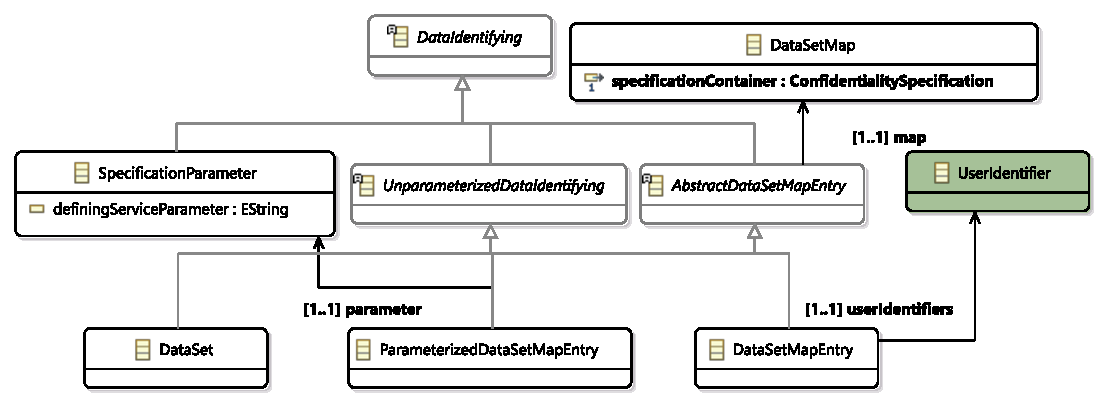
\includegraphics[width=0.9\textwidth]{images/new/data.pdf}
	\caption{Genauere Modellierung des DataSetMapEntry}
\end{figure}
\subsection{System}
Im Package System wurde in der Klasse DataSetMapParameter2KeyAssignment das Attribute assigendKey von einem String zu einer Referenz zu UserIdentifier geändert \ref{systemPackage} Im bisherigen Modell wurde hier der Name eines DataSetMapEntry eingetragen. Durch die Änderung wurde die Beziehung zwischen dem DataSetMapEntry und der DataSetMapParameter2KeyAssignment explizit modelliert. Dies Klasse modelliert, dass ein Connector ein User authentifiziert und ein bestimmten SpecificationParameter zu weißt. Die Stereotype InformationFlowParameterEquation und InformationFlowParameterAssignment wurden entfernt, indem den Klassen SpecificationParameterEquation und AbstractSpecifiationParameterAssignment jeweils eine Referenz zu einem oder mehreren AssemblyContexten bzw. Connectoren hinzugefügt wurde.
\begin{figure}[htbp]
	\label{systemPackage}
	\centering
	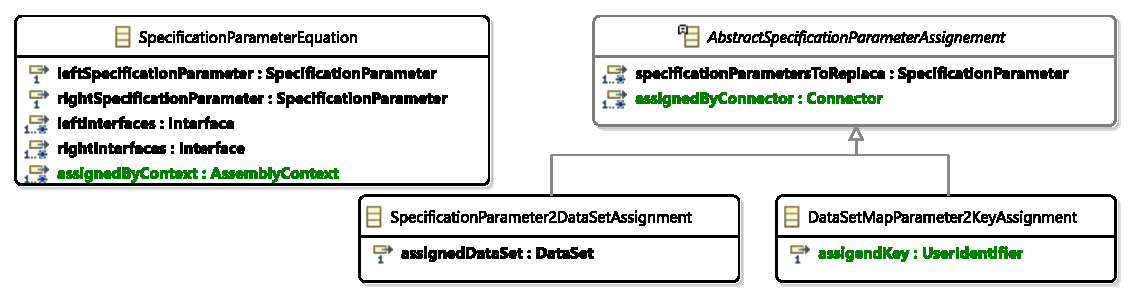
\includegraphics[width=0.9\textwidth]{images/new/system.pdf}
	\caption{Referenzierung des UserIdentifiers}
\end{figure}
\begin{figure}[htbp]
	\label{systemProfil}
	\centering
	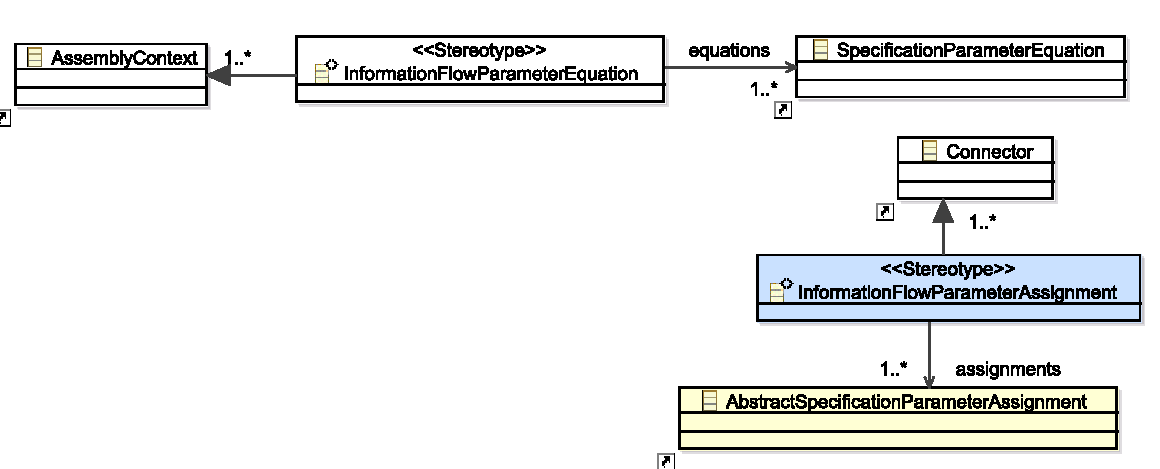
\includegraphics[width=0.8\textwidth]{images/old/systemProfile.pdf}
	\caption{Referenzierung des UserIdentifiers}
\end{figure}

\subsection{Repository}
Der InformationFlow Stereotyp weist Interfaces oder Signatures ParameterAndDataPairs zu. Diese wiederum weisen ein oder mehrere DatenSets bestimmte Informationen dieser Schnittstellen oder Methoden zu, indem der String parameterSource entweder der Name eines Parameter oder $\backslash$call, $\backslash$return, * (alle Information) oder sizeof(<parameterSourceString>) ist. Diese Modellierung ist ungenau insbesondere, wenn mehrere Parameter den selben Namen haben, deshalb wurde im neuen Modell ein weiteres Paket Information \ref{informationPackage} eingeführt, das die ParameterAndDataPair Klasse ersetzen soll. Die abstrakte Klasse Information repräsentiert hierbei ein ParameterAndPair welche jedoch nur noch eine parameterSource haben kann. Diese Einschränkung wurde vorgenommen, da so die Unterklassen direkt den ParameterSource Wert ersetzen können z.B. ersetzt die Klasse CallInfomation ein ParamterAndDataPair mit der ParameterSource $\backslash$call. Die Klasse PararameterInformation  hat jetzt eine explizite Referenz auf einen Parameter. Diese Variante wurde gewählt, da in keinem der Beispiele mehr als eine ParameterSource für ein ParameterAndDataPair definiert wurde sondern immer mehre ParameterAndDataPairs erstellt wurden die teilweis die gleichen DataTargets haben und auf die gleiche Signatur angewandt wurden. \\
Der InformationFlow Stereotyp wurde entfernt indem eine abstrakte Klasse AbstractInformationFlow eingeführt wurde die mehrere Information Instanzen referenzieren kann und je nach Unterklasse auf ein Interface oder eine Signatur verweist. Im alten Modell konnte ein InformationFlow auch auf mehre Signaturen angewandt werden, dies ist im neuen Modell nicht vorgesehen, da die Information wie z.B. CallInformation für jede Signatur andere Informationen sind und deshalb als eigene Instanz der Klasse modelliert werden sollte und Referenzen zu Parameter nur sinnvoll sind wenn der InformationFlow auch nur auf die Signatur oder Interface dieses Parameters angewendet wird. \\
Die Stereotypen ServiceParameterAddition und InformationFlowParameter werden entfernt, indem die neue Klasse InformationFlowParameter einem AbstractInformationFlow einen AddedServiceParameter und mehrere SpecifiactionParamter zu weisen kann.
\begin{figure}[htbp]
	\label{repositoryPackage}
	\centering
	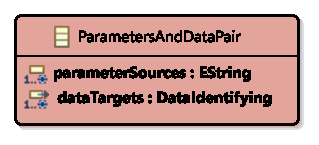
\includegraphics[width=0.19\textwidth]{images/old/repository.pdf}
	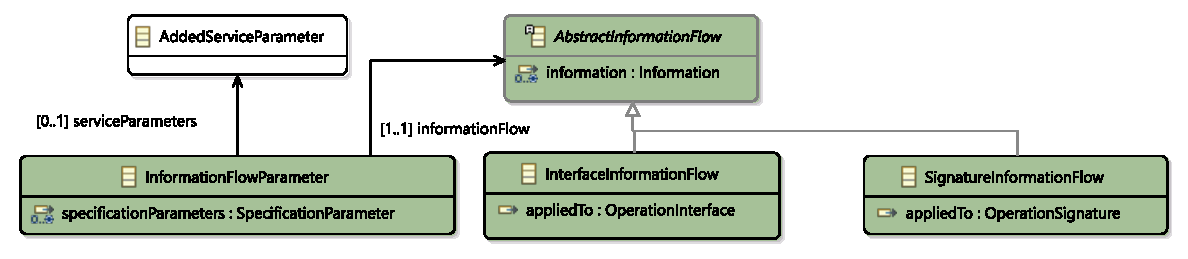
\includegraphics[width=0.77\textwidth]{images/new/repository.pdf}
	\caption{Referenzierung des UserIdentifiers}
\end{figure}
\begin{figure}[htbp]
	\label{informationPackage}
\centering
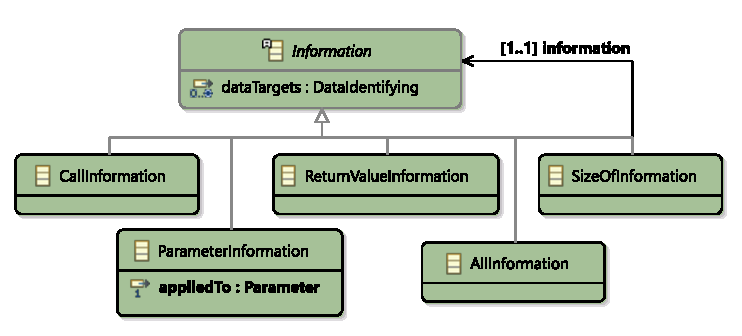
\includegraphics[width=0.8\textwidth]{images/new/information.pdf}
\caption{Referenzierung des UserIdentifiers}
\end{figure}
\begin{figure}[htbp]
	\label{repositoryProfil}
	\centering
	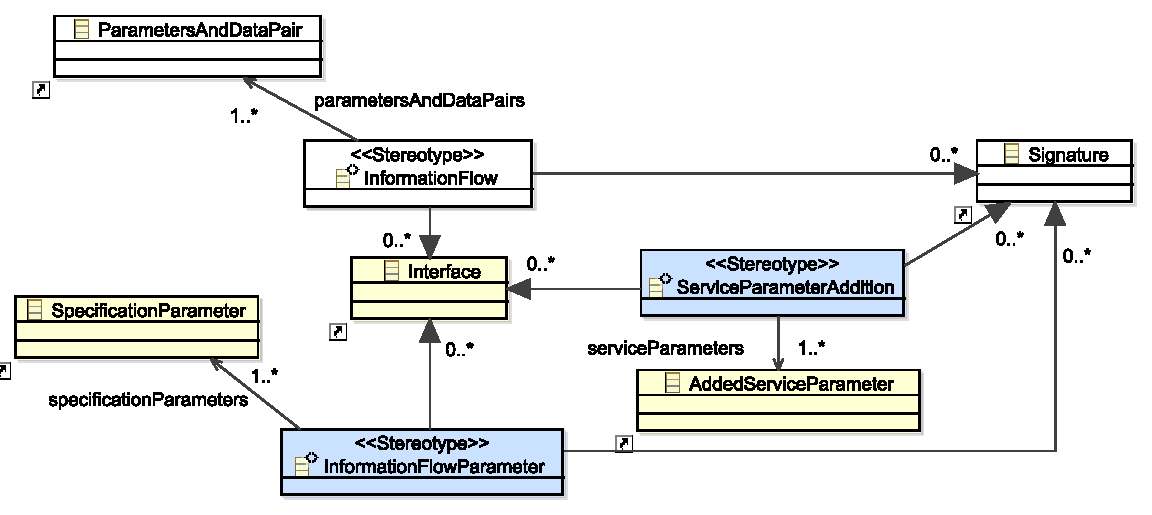
\includegraphics[width=0.8\textwidth]{images/old/repositoryProfile.pdf}
	\caption{Referenzierung des UserIdentifiers}
\end{figure}
\subsection{Resources}
Die Stereotypen Sharing und FutherPhysicalConnections \ref{resoucresProfil} wurde durch die Klasse ResourceContainerConfidentiality ersetzt. Der Stereotyp Encryption \ref{resoucresProfil} wird ersetzt durch die Klasse Encryption. Die Klasse LocationsAndTemperProtectionsPair wird zur abstrakten Klasse AbstraktResourceProtection, deren Unterklassen LinkingResourceProtection und ResourceContainerProtection referenzieren auf LinkingResources bzw. ResourceContainer, sodass der Stereotyp LocationAndTamperProtection nicht mehr benötigt wird. Allerdsings kann eine AbstraktResourceProtection Instanz jetzt nur noch entweder auf LinkingResoucres oder auf ResourceContainer verweisen nicht mehr auf beides gleichzeitig.
\begin{figure}[htbp]
	\label{resoucresPackage}
	\centering
	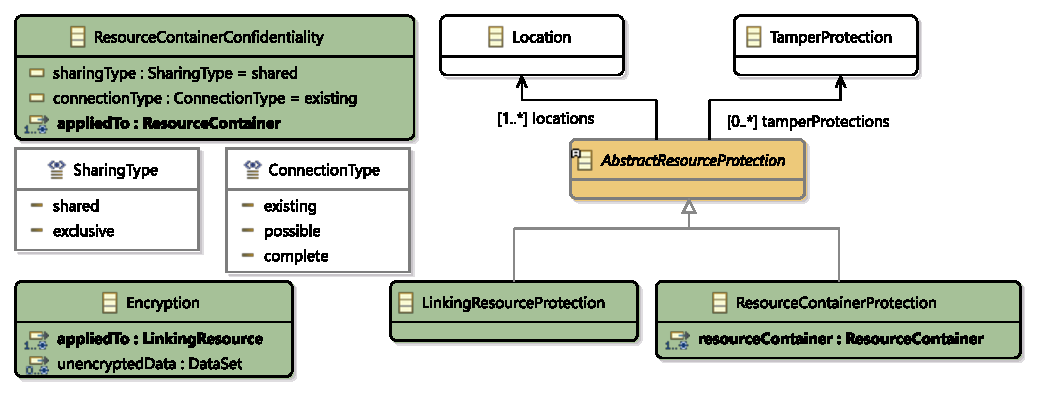
\includegraphics[width=0.9\textwidth]{images/new/resources.pdf}
	\caption{Referenzierung des UserIdentifiers}
\end{figure}
\begin{figure}[htbp]
	\label{resoucresProfil}
	\centering
	\includegraphics[width=0.99\textwidth]{images/old/resourceProfile.pdf}
	\caption{Referenzierung des UserIdentifiers}
\end{figure}

\subsection{Adversary}
Das Adversary Paket hat sich nur dadurch verändert, dass nur die Reference mayTamperWith nicht mehr auf die Klasse LocationAndTamperProtectionsPair zeigt, sondern auf die KlasseAbstractResourceProtection.
\begin{figure}[htbp]
	\label{adversaryPackage}
	\centering
	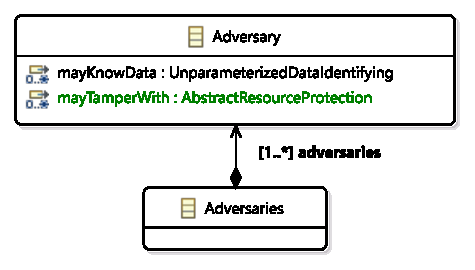
\includegraphics[width=0.4\textwidth]{images/new/adversary.pdf}
	\caption{Referenzierung des UserIdentifiers}
\end{figure}

\begin{itemize}
	\item Profile entfernt
	\item Genauere Modellierung des Informationsflusses
	\item Identifier aus PCM
\end{itemize}


\section{PCM2Prolog Generator}
Der PCM2Prolog Generator wandelt eine Instanz des Confientiality Modells in Prolog Prädikate um. Dieser musste im Rahmen dieses Projekts so angepasst werden, dass trotz des veränderten Modells der Prolog Code identisch ist. \\ \\
Grundsätzlich verwendet der Generator die Reflective API von ECore und ist in xTend geschrieben. Für jedes Entität wird die Methode \texttt{String generateDeeply(EObject e)} aufgerufen. Diese generiert für jedes Object und dessen Kinder PrologPrädikate für alle Referenzen und Attribute. Der Form:
\texttt{referenceName(''objId'', [''refObjId1'',''refObjId2'']).} \\ In der Klasse \textit{PCM2PrologXSBFilter} kann hierbei angegeben werden welche Klassen und Referenzen berücksichtigt werden sollen. \\ \\
Für Objekte die nicht automatisch generiert werden können, können Dispatch-Methoden für die  \texttt{String generateDeeply(EObject e)} Methode definiert werden. Dies wurde für viele der neu hinzugefügten Klassen gemacht, um sicherzustellen, dass die Prolog Prädikate identisch zum ursprünglichen Modell sind.\\ \\
Durch das entfernen des Profil-Mechanismus hat sich die Richtung der Referenzen der PCM Komponenten zu den Veraulichkeitsinformationen umgedreht. Im ursprünglichen Modell hat ein Stereotype wie z.B. LocationAndTemperProtection angewandt auf einen ResourceContainer mehrere LocationAndTemperProtectionPairs und wird in ein einziges Prädikat umgewandelt. Im neuen Modell gibt es allerdings für jedes LocationAndTemperProtectionPair eine ResourceContainerProtection mit einer Referenz auf den enspechenden ResourceContainer. Damit diese Referenzen trotzdem in ein Prädikat pro ResourceContainer umgesetzt werden können, werden die Referenzen in einer Map gespeichert wobei der Identifier des ResourceContainers als Key dient. So kann nach dem alle Objekte verarbeitet wurden, für jeden ResourceContainer in der Liste ein Prädikat generiert werden mit den entsprechenden Identifieren der zugehörigen ResourceContainerProtections. Das selbe Prinzip wird auch für die SpecificationParameterEquation, InformationFlowParameter und AbstractInformationFlows benötigt.

\section{Evaluierung}
Um zu überprüfuen ob der generierte Prolog Code identisch zu dem Prolog Code vor der Refaktorisierung ist wurden die Beispiel Projekte Cloud-minimzied\footnote{https://github.com/KASTEL-SCBS/Examples4SCBS/tree/master/bundles/edu.kit.kastel.scbs.cloudscenario-minimized} und IFlowExample\footnote{https://github.com/KASTEL-SCBS/Examples4SCBS/tree/master/bundles/edu.kit.kastel.scbs.iflowexample} im neuen Modell modelliert und das Ergebnis mit dem Ergebnis des ursprünglichen Modells vergleichen. Diese zwei Beispiel Projekte wurden gewählt, da sie gemeinsam nahe zu alle Elemente des Confientiality Modells abdecken. Die einzige nicht verwendet Klasse ist die SpecificationParameter2DataSetAssignment Klasse. Diese wurde gesondert händisch getestet. \\
%
Um den Prolog Code automatisch vergleichbar zu machen müssen beim Modellieren die selben Identifier verwendet werden wie in original Projekt. Die Identifier der LocationAndTemperProtectionsPair Elemente müssen identisch zu den Identifierer der AbstractResourceProtection Elemente sein. Die Identifier der ParameterAndDataPair Elemente müssen identisch zu den Identifiern der Information Elemente sein. Die Identifier der anderen neuen Klassen können frei gewählt werden. \\ \\
Beim generieren des Prolog Codes die Option fullIDs, singleFile und noComment ausgewählt werden, da bewusst die Kommentare nicht identisch sind, sondern so, dass auf die Entitäten aus denen die Prolog Prädikate generiert wurden zurück geschlossen werden kann. \\ \\
Im letzten Schritt müssen die Ausgabe Dateien noch vereinheitlicht werden. Dies ist jediglich notwendig um die die Dateien automatisch vergleichen zu können. Es gibt viele Prädikate der Form: \\ \\ \texttt{prädikatName(''entity'',[''child1'',''child1'',''child3'']).} \\ \\ Die Reihenfolge der Elemente \texttt{child1} bis \texttt{child3} in der Liste ist hierbei irrelevant. Deshalb müssen die Listenelemente solcher Prädikate alphabetisch sortiert werden. Außerdem kann sich die Reihenfolge der Zeilen in unterscheiden. Deshalb wird anschließend die Datei zeilenweise sortiert und leere Zeilen entfernt. Diese beiden Schritte können mit einem einfachen Shell Skript durchgeführt werden. 
Auf den vereinheitlichen Dateien kann dann ein diff ausgeführt werden. \\ \\
Beide Beispiel Projekte CloudScenario-minimized udn IflowExample konnten erfolgreich so im neuen Modell modelliert werden, dass der Prolog Code identisch ist. Allerding mussten im CloudScenario-minimized Beispiel eine kleine Änderung vorgenommen werden, da eine Referenz auf ein LocationAndTemperProtectionsPair in cloud.adverary zwar defninert war aber nicht im cloud.confidentielity File. In IFlowExample gab es  undefinierte Referenzen innerhalb der Elementen \textit{Allocation Energy Visualization}, \textit{Allocation Database DBMS} und \textit{Allocation Energy Meter} im File \textit{default.allocation} und innerhalb der Elemente \textit{ProvDelegation Provided AnInterface -> Provided AnInterface AComponent}, \textit{Connector Energy Visualization -> Database} und \textit{Connector Energy Visualization -> Energy Meter Assembly Context} und im \textit{default.system} File. Da diese Elemente in in der Vertraulichkeitsanalyse referenziert werden, konnten diese gelöscht werden. Das Problem der undefinierten Referenzen ist, dass diese beim Generieren des Prolog Codes zu Prädikaten mit zufälligen Identifiern führen. 
%% --------------------
%% |   Bibliography   |
%% --------------------

%% Add entry to the table of contents for the bibliography
%\printbibliography[heading=bibintoc]
\printbibliography

\end{document}